\documentclass{article}
\usepackage{tikz}
\usepackage{pgfplots}
\pgfplotsset{width=7cm,compat=1.5.1} 
\begin{document}
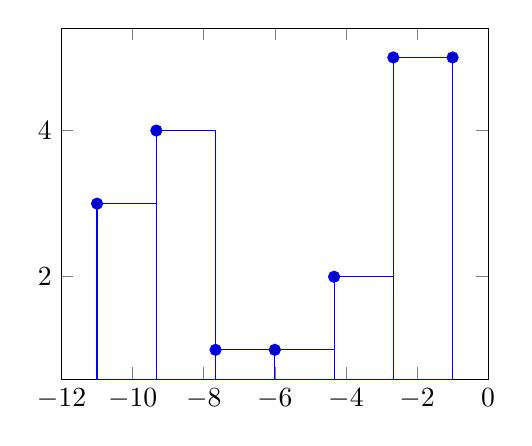
\begin{tikzpicture} 
\begin{axis}[
  %ybar interval,
  %xticklabel=
%\pgfmathprintnumber\tick--\pgfmathprintnumber\nexttick
]
    \addplot+[hist={bins=6}]
        table[row sep=\\,y index=0] {
        data\\
        -1\\ -2\\ -1\\ -5\\ -4\\ -10\\
        -7\\ -10\\ -9\\ -8\\ -9\\ -9\\ -11\\ -1\\ -3\\ -2\\
    };
\end{axis}
\end{tikzpicture}


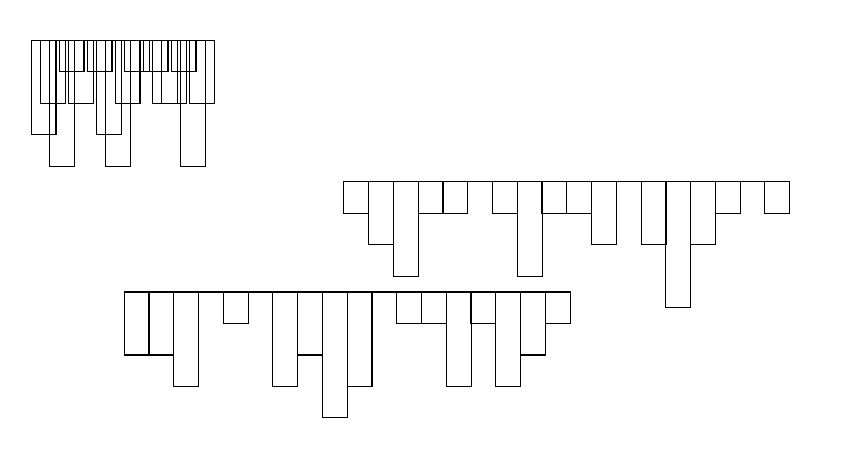
\begin{tikzpicture}
\begin{axis}[
   at={(0.36\linewidth,0)},
   ybar, 
   bar width=9pt,
   width=4cm, 
   height=3.5cm,
   axis lines=none
   ]
\addplot[fill=white]%
 coordinates {
  (0,-3) (1,-2) (2,-4) (3,-1) (4,-2) (5,0) 
  (6,-1) (7,-3) (8,-4) (9,-2) (10,-1) (11,0) 
  (12,-1) (13,-2) (14,-2) (15,-1) (16,-4) (17,-2)
  };
\end{axis}
%
\begin{axis}[
   at={(0.66\linewidth,-450)},
   ybar, 
   bar width=9pt,
   width=8cm, 
   height=3.5cm,
   axis lines=none
   ]
\addplot[fill=white]%
 coordinates {
   (0,-1) (1,-2) (2,-3) (3,-1) (4,-1) (5,0) 
  (6,-1) (7,-3) (8,-1) (9,-1) (10,-2) (11,0) 
  (12,-2) (13,-4) (14,-2) (15,-1) (16,0) (17,-1)
 };
\end{axis}
%
\begin{axis}[
   at={(0.43\linewidth,-800)},
   ybar, 
   bar width=9pt,
   width=8cm, 
   height=3.5cm,
   axis lines=none
   ]
\addplot[fill=white]%
 coordinates {
   (0,-2) (1,-2) (2,-3) (3,-0) (4,-1) (5,0)
  (6,-3) (7,-2) (8,-4) (9,-3) (10,0) (11,-1) 
  (12,-1) (13,-3) (14,-1) (15,-3) (16,-2) (17,-1) 
 };
\end{axis}
\end{tikzpicture}



\end{document}
